\documentclass[a4paper, 10 pt, conference]{ieeeconf}
\overrideIEEEmargins
\usepackage{polski}
\usepackage{amsmath}
\usepackage{graphicx}
\usepackage[utf8]{inputenc}
\usepackage[T1]{fontenc}
\usepackage{textcomp}
\usepackage[english]{babel}
\usepackage{hyperref}

\newcommand{\bb}{\textbf}

% Listingi
\usepackage{listings}
\usepackage{xcolor}
\lstdefinestyle{mystyle}{
	backgroundcolor=\color{gray!5!white},
	commentstyle=\color{green!50!black},
	keywordstyle=\color{magenta},
	numberstyle=\tiny\color{black!50!white},
	stringstyle=\color{purple},
	basicstyle=\footnotesize,
	breakatwhitespace=false,
	breaklines=true,
	captionpos=b,
	keepspaces=true,
	numbers=left,
	numbersep=5pt,
	showspaces=false,
	showstringspaces=false,
	showtabs=false,
	tabsize=2
}
\lstset{style=mystyle}

% The following packages can be found on http:\\www.ctan.org
\usepackage{graphics} % for pdf, bitmapped graphics files
\usepackage{amsmath} % assumes amsmath package installed
\usepackage{amssymb}  % assumes amsmath package installed
\usepackage{tikz}
\usetikzlibrary{positioning} 
\usepackage{makecell}

\title{\LARGE \bf
Analysis of the effectiveness of recursive
networks in the classification task
}

\author{\parbox{2 in}{\centering Paweł Ksieniewicz \\
        Wrocław University of Science and Technology\\
        {\tt\small pawel.ksieniewicz@pwr.edu.pl}}
        \hspace*{ 0.3 in}
        \parbox{2 in}{\centering Jędrzej Kozal \\
        Wrocław University of Science and Technology\\
        {\tt\small 218557@student.pwr.edu.pl}}
}


\begin{document}

\maketitle
\thispagestyle{empty}
\pagestyle{empty}

\selectlanguage{english}
\begin{abstract}

Recurrent Neural Networks are class of models designed to process sequences. Most of typical fields of applications include natural language processing, recognition of handwriting and generation of text, music or images. In this work emphasis was put on a ReNet architecture designed to solve an image classification task. A modification based on a Hilbert curve was introduced to the ReNet and obtained accuracy was very close to results acquired for the original ReNet network. The modification also provided significant training time reduction for some datasets. Comparison of ReNet networks to convolutional networks proved that the latter are superior.

\end{abstract}


\section{INTRODUCTION}



 

\section{RELATED WORK}

In \cite{DBLP:journals/corr/VisinKCMCB15} ReNet architecture was introduced. It is alternative to convolutional networks, that enables to learn representation of an image, that can be used for classification purpose. Convolutional network computes activation based on the filters applied locally to part of an image. ReNet by using 4 recurrent neural networks can incorporate information scattered across whole image.

For convenience from now on we will refer to input as an image, but it can be also output of previous layer. We can describe inputs as tensor $X = \{x_{i,j}\}, X \in \mathbb{R}^{w \textrm{x} h \textrm{x} c}$, where $w, h$ are size of an image and $c$ is a number of channels. Image is divided into block of pixels called patches. Every patch is of size: $w_p$, $h_p$, therefore there are $(I \times J),I=\frac{w}{w_p}, J=\frac{h}{h_p}$ patches in the whole image. Set of all patches in image $X$ is defined as $P = \{p_{i,j}\}, P \in \mathbb{R}^{w_p \textrm{x} h_p \textrm{x} c}$. In first part of ReNet algorithm we take each columns of patches and feed it to 2 recurrent neural networks: 

\begin{gather}
	v_{i,j}^{F} = f_{VFWD} (v_{i,j-1}^F, p_{i,j}), \\
    v_{i,j}^{R} = f_{VREV} (v_{i,j+1}^R, p_{i,j}),
\end{gather}

where $f_{VFWD} (v_{i,j-1}^F, p_{i,j})$ can be activation of plain RNN, LSTM cell or GRU cell. Concatenated activation can be described as $V = \{v_{i,j}\}_{i=1,...,I}^{j=1,...,J}$. Tensor $V$ is input of another two recurrent layer networks, swapping rows from left to right, and right to left. Operation is analogues to vertical swap, with $f_{HFWD}, f_{HREV}$ computing activations $H = \{h_{i,j}\}$. Transformation $\Phi$ of each layer can be described with introduced designation as:

\begin{equation}
	\Phi: X \rightarrow V \rightarrow H
\end{equation}

Output of layer can be feed to another ReNet layer, or can flatted and feed to fully connected layer.

\section{METHODS}

\subsection{Hilbert curve}

\begin{figure}
	\centering
	\begin{tikzpicture}
	\draw (0,0) node[below] {1} -- (0,2) node[above] {2} -- (2,2) node[above] {3} -- (2,0) node[below] {4};
	\draw (0,2.5) node[above] {1} -- (0.66,2.5) node[above] {2} -- (1.32,2.5) node[above] {3} -- (2,2.5) node[above] {4};
	\draw (3,0) node[below] {1} -- (3.75,0) node[below] {2} -- (3.75,0.75) -- (3,0.75) -- (3,1.5) -- (3,2.25) -- (3.75,2.25) -- (3.75,1.5) -- (4.5,1.5) -- (4.5,2.25) -- (5.25,2.25) -- (5.25,1.5)  -- (5.25,0.75) -- (4.5,0.75) -- (4.5,0) -- (5.25,0);
	\draw (6.25,0) -- (6.25,0.4);
	\end{tikzpicture}
\caption{First 3 elements of sequence creating Hilbert Curve.}
	\label{fig:hilbert}
\end{figure}

Hilbert Curve $\mathcal{H}$ is space filling curve with fractal structure. It is defined by sequence of curves defined recursively, what be described as $k(n+1) = f(k(n))$. In this case transformation $f$ compounds of duplicating and rotating of $n$-th degree curve. First 3 elements of sequence creating Hilbert Cureve are shown in figure \ref{fig:hilbert}.

We can obtain Hilbert Curve in limit:

\begin{equation}
	\mathcal{H} = \lim_{n \rightarrow + \infty } k(n)
\end{equation}

By doing so, we can fill every point of unit square, hence name of this mathematical object - space filling curve. Hilbert Curve have other interesting quantities. $N$-th curve from sequence defining Hilbert Curve provides method of traversing image with side of length $2^{N}$. This can be utilized to define mapping from 2D to 1D and inverse. This mapping have one useful property. The same regions of an image are mapped to similar segments of line, regardless what the degree of this curve is. For graphical demonstration see lines above each curve in figure \ref{fig:hilbert}.

\subsection{ReNet modification}

We can utilize mapping defined by Hilbert Curve to reduce dimensionality of image. Then we can reduce number of recurrent neural networks in each ReNet layer. Instead of 4 RNN swapping image columns and rows we can introduce 2 RNN swaping image converted to 1D sequence with Hilbert Curve.

We can define image after mapping to 1D as: $x^{h} = \mathcal{H}(x)$. To keep reduction of activation dimensions after each modified ReNet layer we introduce patches as in original ReNet. In this case patch is defined as set of subsequent pixels: $P^{h} = \{ p_{i}^h \}$, $P^{h} \in \mathbb{R}^{w_p \textrm{x} c}$. As in original ReNet pixels from same patch are one input of recurrent neural network. If patch size is 1, then RNN in modified ReNet layer works as bidirectional recurrent neural network. Activations of whole layers are concatenation of 2 RNN activations:

\begin{gather}
	v_{i}^{F} = f_{FWD}(v_{i-1}^{F}, p_{i}^{h}) \\
	v_{i}^{R} = f_{REV}(v_{i+1}^{F}, p_{i}^{h})
\end{gather}

To further speedup the computations, subsequent modified ReNet layers use activation provided by previous layer. No mapping or inverse mapping is needed.

By using Hilbert Curve we mean to hold some spatial information while reducing image size. By aplaying image size reduction introduced by patches, segments of activations sequence still correspond to fragments of image. This should reduce impact of reducing dimensionality of the data.

\section{EXPERIMENT SETUP}

In order to provide valid comparison of previously described method accuracy of ReNet, ReNet with modifcation and convolutional neural network was measured. For traning of all networks Adam optimization method was emplyed. 

\subsection{Datasets}

\begin{table}
\centering
\caption{Datasets used for experiments}
\label{tab:dataset}
\begin{tabular}{ |c|c|c|c|c|c| } 
 \hline
 dataset & \#images & \#classes & width & height & source \\ 
 \hline
 \makecell{Chest X-Ray\\ Images (Pneumonia)} & 5863 & 2 & \textnormal{>}1500 & \textnormal{>}1000 & \cite{xray-dataset}\\ 
 \hline
 \makecell{Flowers Recognition} & 4242 & 5 & 320 & 240 & \cite{flowers-dataset} \\ 
 \hline
 \makecell{Fashion MNIST} & 70000 & 10 & 28 & 28 & \cite{fashion-dataset} \\ 
 \hline
 \makecell{Natural Images} & 6899 & 8 & \textnormal{>}200 & \textnormal{>}50 & \cite{natural-img-dataset} \\ 
 \hline
\end{tabular}
\end{table}

Comparison of used datasets is given in table \ref{tab:dataset}. Chest X-Ray, Flowers Recognition and Natural Images datasets were downloaded with usage of kaggle public API in version respectively 2, 2 and 1. Fashion MNIST dataset was downloaded using keras library. In case of x-ray dataset conversion to greyscale was applied. All images were resized to (64,64) or (32,32) size, due to issues with to low GPU memory when using ReNet networks on larger images. This limits the field of application of ReNet to small images only.

\subsection{Used tools and hardware}

Experiments were performed using Google Colab, Google Clound Platform with usage of AI Platform and local PC with IntelCore i7 8700 processor and graphic card GTX 1070Ti. Code was implemented using keras library with tensorflow backend. Scikit-learn and numpy were also used.

\subsection{Hyperparameters finetuning}

To choose best model structure and hyperparameters modified version of Grid Search was applied. In normal setup Grid Search is complete search of defined hyperparameters space. Instead of complete search greedy search was introduced. Each value of hyperparameter was chosen separately. Order of choosing hyperparams was as follows: learning rates and regularization terms, then number of ReNet or convolutional layers with dropout probability, number of neurons in ReNet or convolutional layers and finally number of neurons in fully conected layers with dropout probability. This is a naive approach because we assume independent influence of controlled factors on process of learning. 

\section{RESULTS}

\subsection{Quantitative results}

\begin{table}[ht]
    \centering
    \caption{Average accuracy for 5-fold cross validation}
\begin{tabular}{|c|l|l|l|}
  \hline
  dataset & ReNet & modif ReNet & conv \\
  \hline
  \makecell{Chest X-Ray\\ Images (Pneumonia)} & 0.919 & 0.931 & 0.949 \\
  \hline
  \makecell{Flowers Recognition} & 0.538 & 0.553 & 0.657 \\
  \hline
  \makecell{Fashion MNIST} & 0.869 & 0.861 & 0.927 \\
  \hline
  \makecell{Natural Images} & 0.842 & 0.756 & 0.935 \\
  \hline
\end{tabular}
    \label{table:cross_validation}
\end{table}

\begin{table}[ht]
    \centering
    \caption{Comparison of p-values and H-values of Kruskal-Wallis test}
    \begin{tabular}{|c|l|l|}
  \hline
  dataset & wartość statystyki H & p-wartość \\
  \hline
  \makecell{Chest X-Ray\\ Images (Pneumonia)} & 11.579 & 0.003 \\
  \hline
  \makecell{Flowers Recognition} & 10.220 & 0.006 \\
  \hline
  \makecell{Fashion MNIST} & 10.820 & 0.004 \\
  \hline
  \makecell{Natural Images} & 12.5 & 0.001 \\
  \hline
\end{tabular}
    \label{table:kruskal}
\end{table}

\begin{table}[ht]
    \centering
    \caption{Comparison of p-values for Conover post-hoc tests}
    \begin{tabular}{|c|l|l|l|}
  \hline
  dataset & \makecell{ReNet\\ modif ReNet} & \makecell{ReNet\\ conv} & \makecell{modif ReNet\\ conv} \\
  \hline
  \makecell{Chest X-Ray\\ Images (Pneumonia)} & 0.016 & 0.001 & 0.001 \\
  \hline
  \makecell{Flowers Recognition} & 0.189 & 0.001 & 0.001 \\
  \hline
  \makecell{Fashion MNIST} & 0.071 & 0.001 & 0.001 \\
  \hline
  \makecell{Natural Images} & 0.001 & 0.001 & 0.001 \\
  \hline
\end{tabular}
    \label{table:posthoc}
\end{table}

\begin{table}[ht]
    \centering
    \caption{Comparison of average epoch training time for first 100 samples of each dataset}
    \begin{tabular}{|c|l|l|}
  \hline
  dataset & ReNet & modif ReNet \\
  \hline
  \makecell{Chest X-Ray\\ Images (Pneumonia)} & 1.170 & 0.603 \\
  \hline
  \makecell{Flowers Recognition} & 0.324 & 0.157 \\
  \hline
  \makecell{Fashion MNIST} & 0.392 & 0.155 \\
  \hline
  \makecell{Natural Images} & 0.332 & 0.321 \\
  \hline
\end{tabular}
    \label{table:time_avrg}
\end{table}

Average results for a cross validation are presented in a table \ref{table:cross_validation}, results of statistical tests in tables \ref{table:kruskal} and \ref{table:posthoc}. Comparison of a training time is given in a table \ref{table:time_avrg}. Based on a Kruskal-Wallis test with statistical significance level 0.05 one can say that results obtained for all algorithms are significantly different. Based on the post-hoc tests with the same significance level one cane say, that results obtained for ReNet and ReNet with modification are not significantly different for datasets Flowers Recognition and Fashion MNIST.

\subsection{Qualitative results}

\begin{figure*}
\centering
	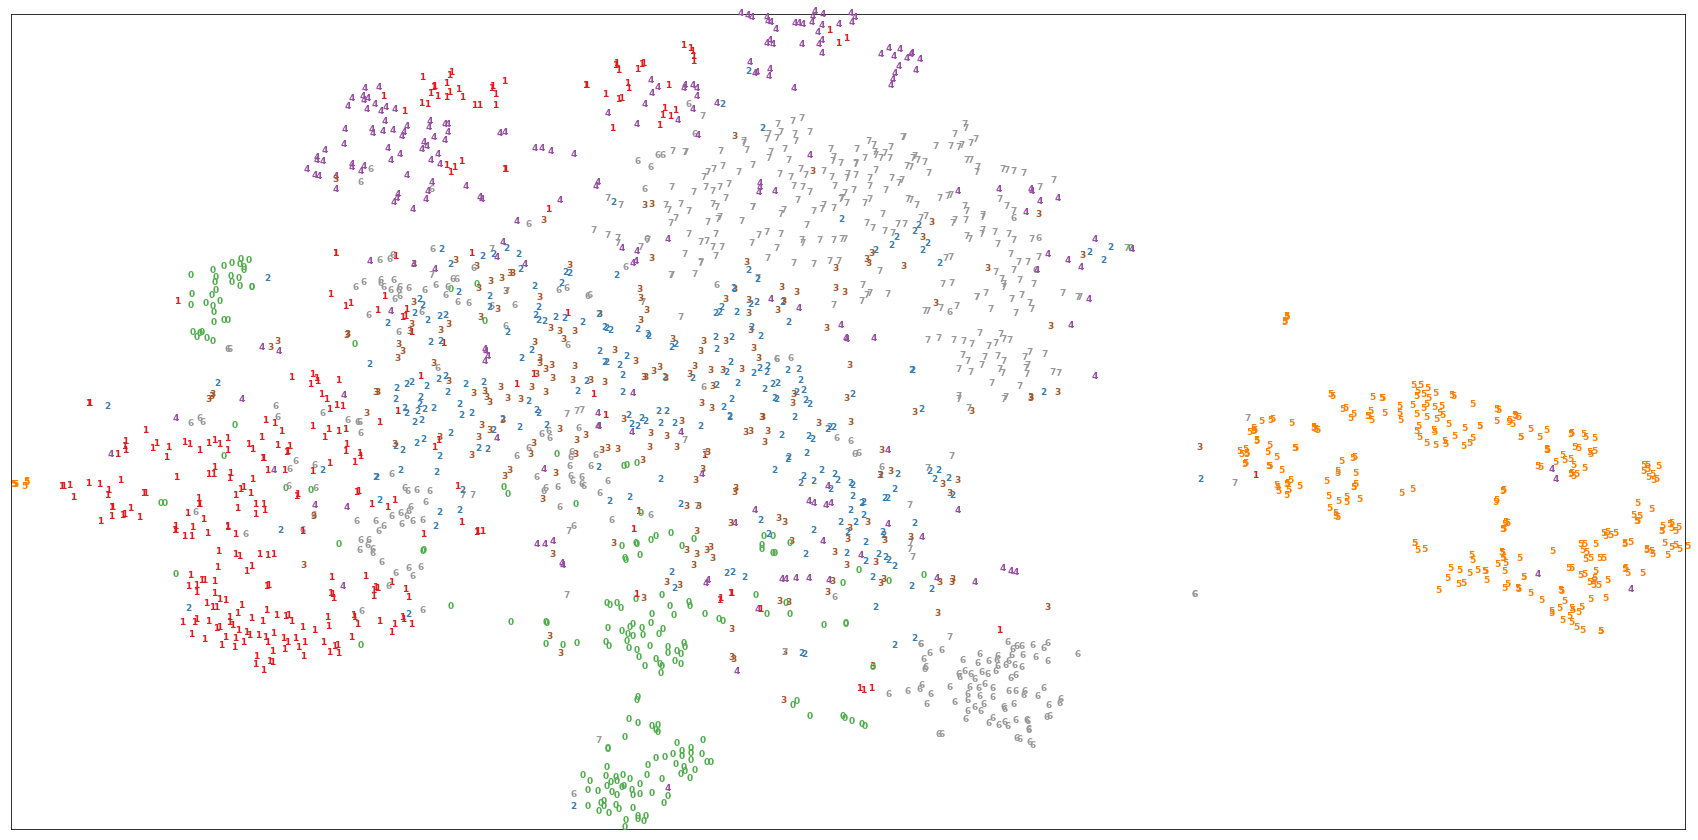
\includegraphics[width=1.0\textwidth]{img/tSNE_ReNet.png}
	\caption{Visualization of representation learned by ReNet network after applying tSNE}
	\label{fig:tSNE_ReNet}
\end{figure*}

\begin{figure*}
\centering
	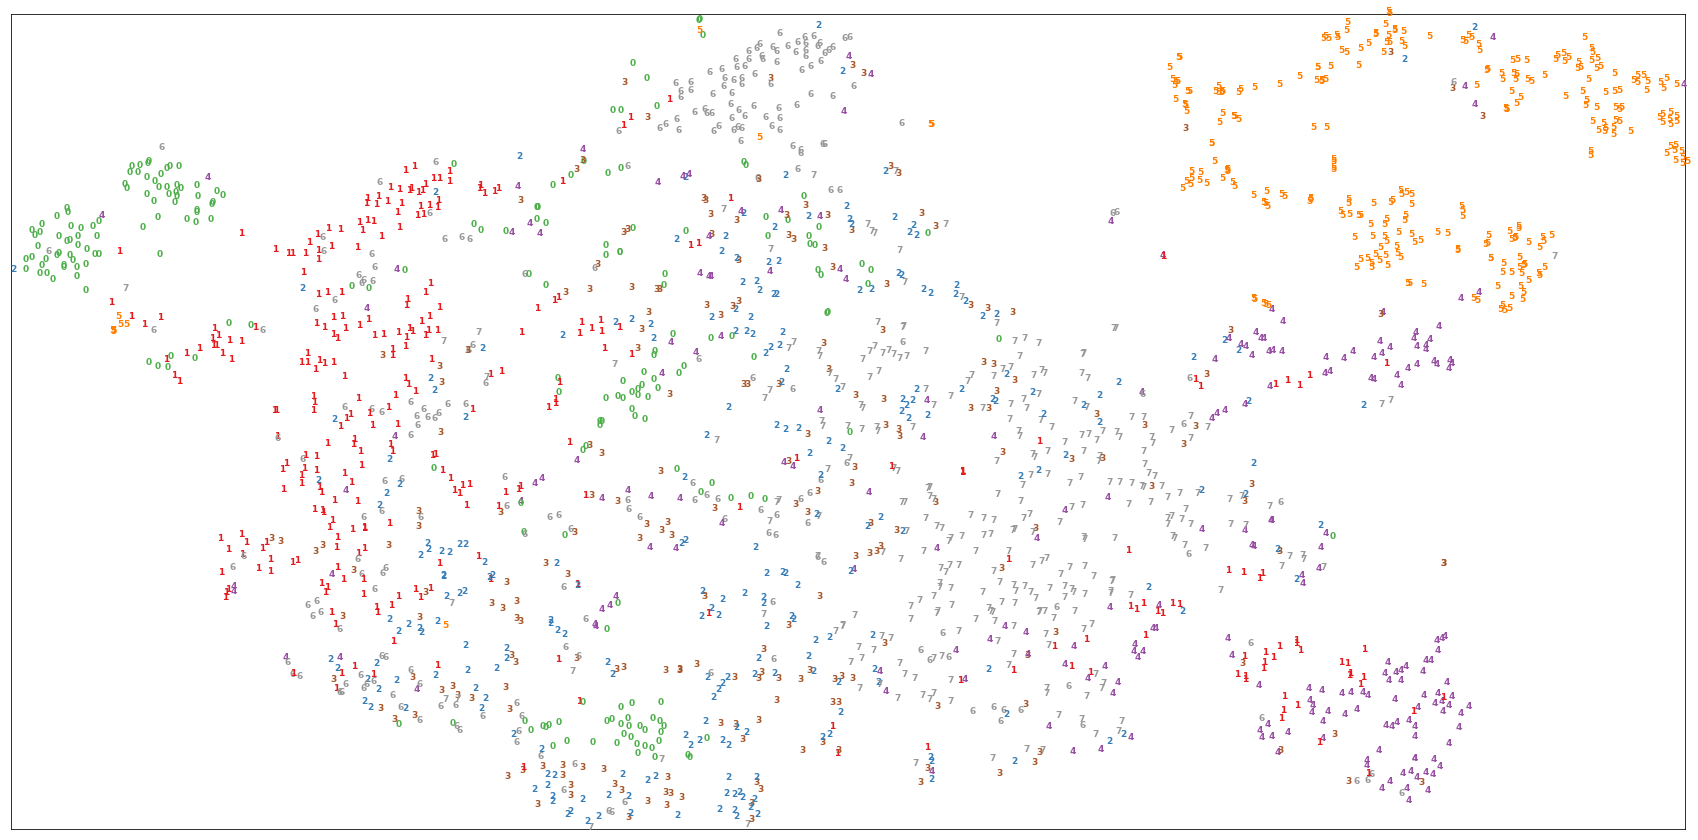
\includegraphics[width=1.0\textwidth]{img/tSNE_modif_ReNet.png}
	\caption{Visualization of representation learned by modified ReNet network after applying tSNE}
	\label{fig:tSNE_modif_ReNet}
\end{figure*}

\begin{figure*}
\centering
	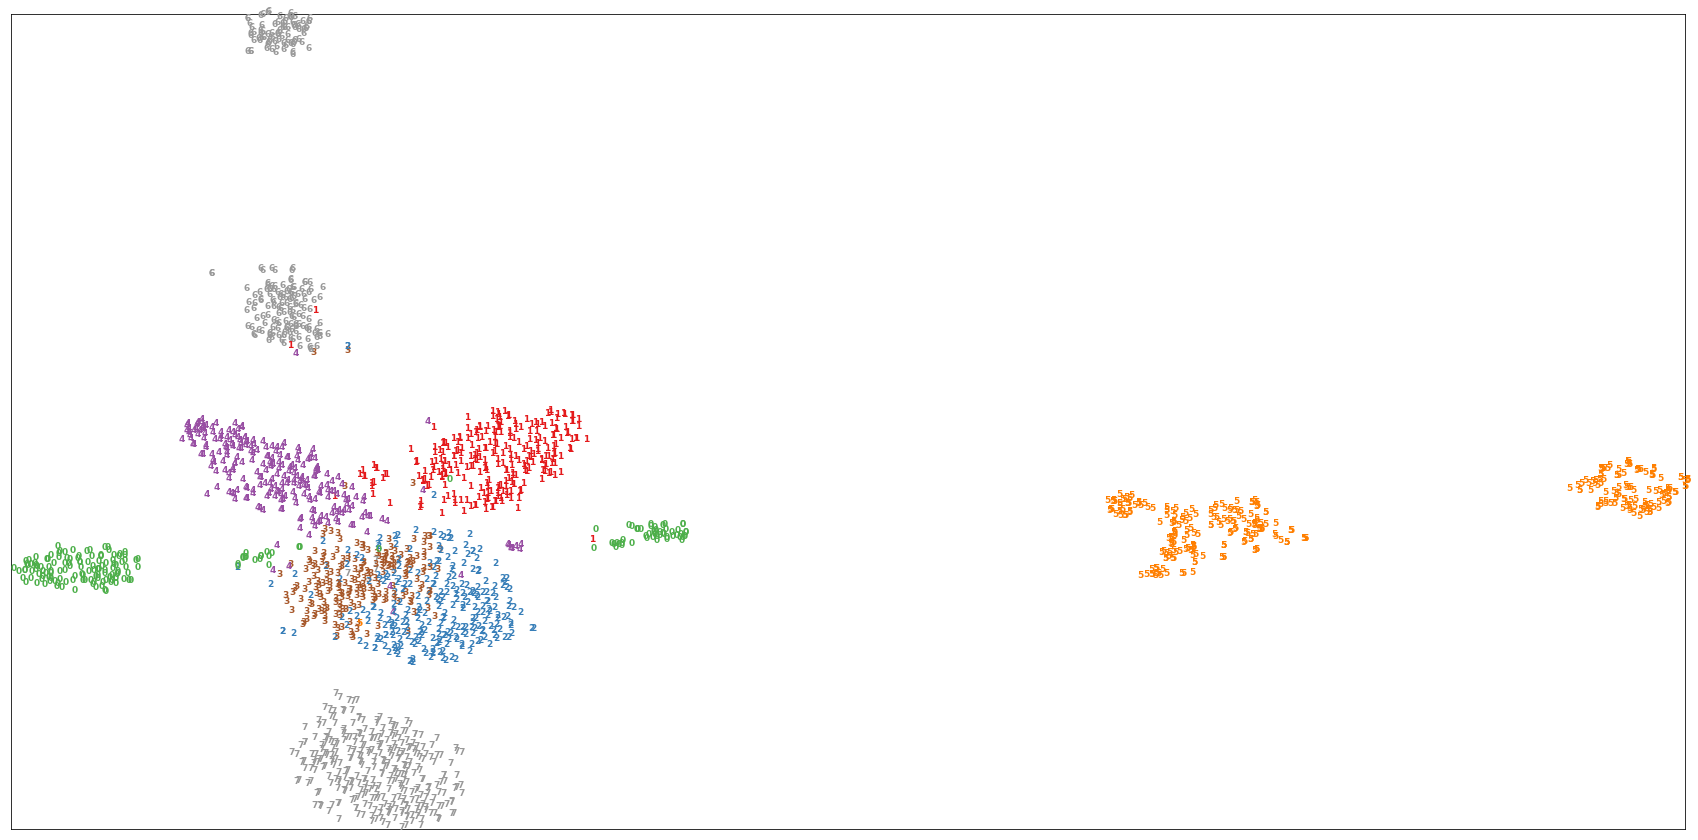
\includegraphics[width=1.0\textwidth]{img/tSNE_conv.png}
	\caption{Visualization of representation learned by convolutional neural network after applying tSNE}
	\label{fig:tSNE_conv}
\end{figure*}

Based on \cite{tSNE} visualization of features learned by network were computed. Here features learned by network are understood as outputs of layer before fully connected layer with softmax activation function. All of this outputs were computed for test set of Natural Images dataset. Results are presented in figures \ref{fig:tSNE_ReNet}, \ref{fig:tSNE_modif_ReNet} and \ref{fig:tSNE_conv}.

\begin{figure*}
\centering
	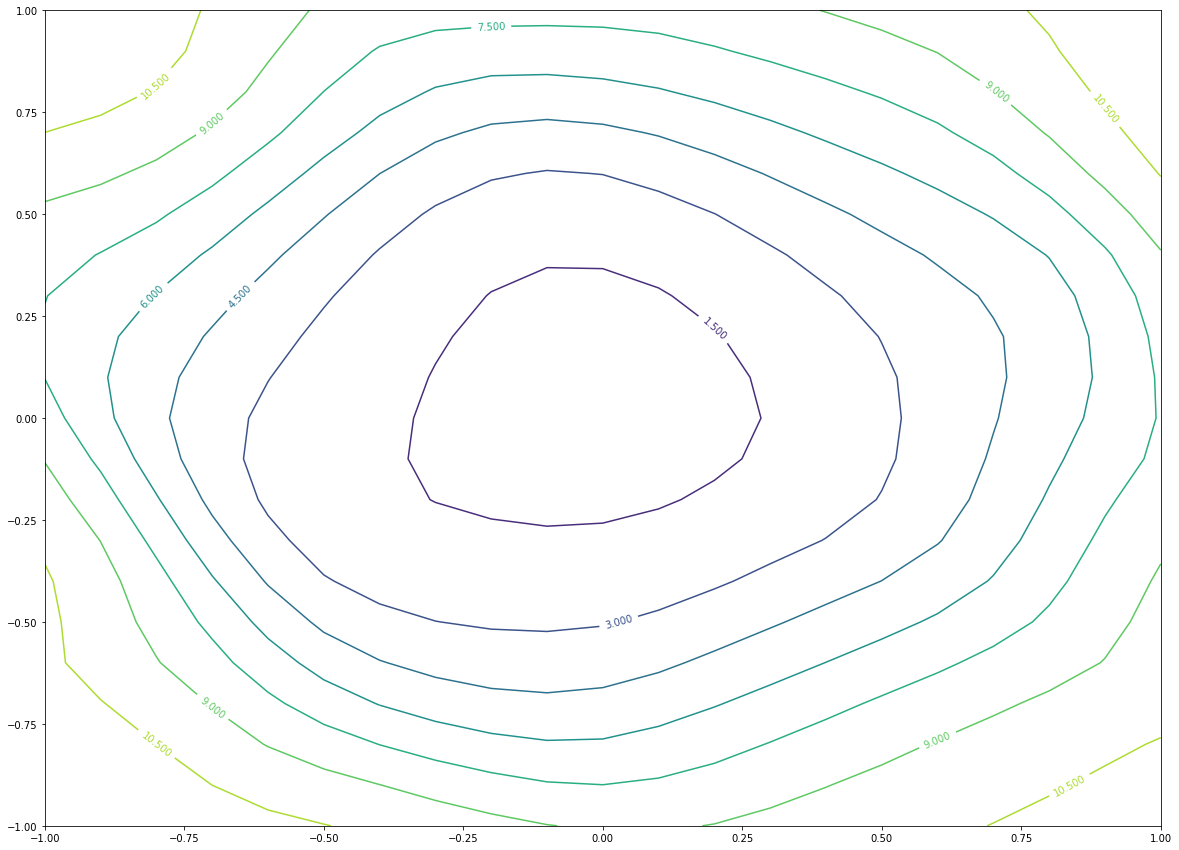
\includegraphics[width=0.49\textwidth]{img/loss_ReNet.png}
	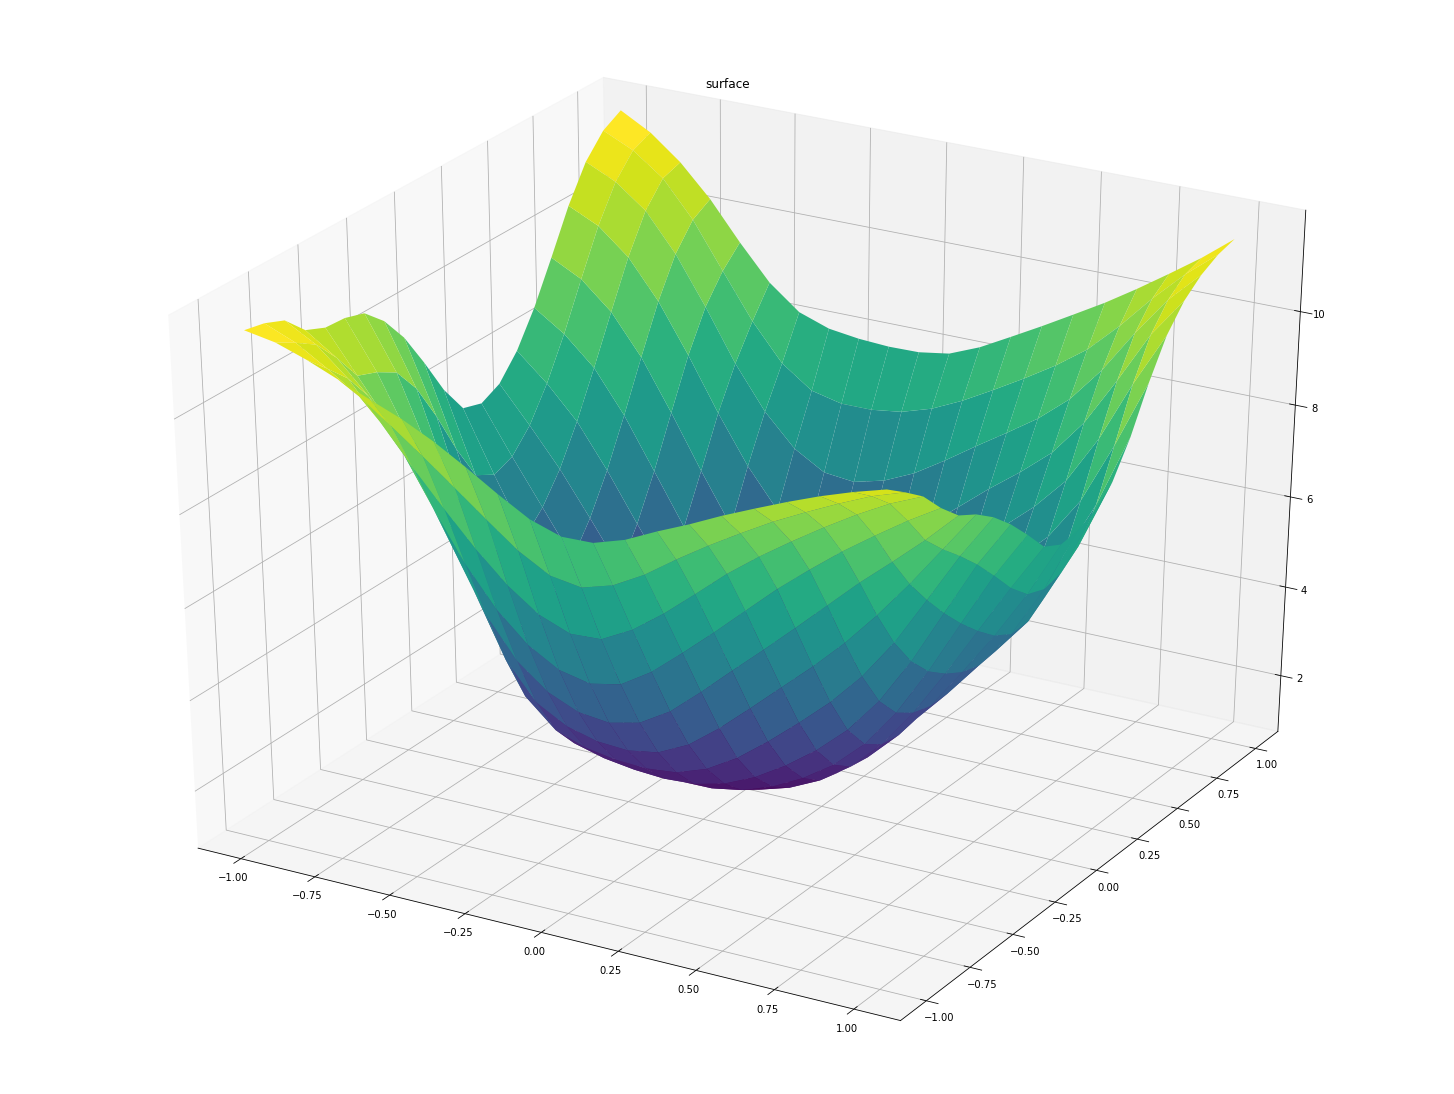
\includegraphics[width=0.49\textwidth]{img/loss_3d_ReNet.png}
	\caption{Visualization of loss landscape of ReNet network}
	\label{fig:loss_ReNet}
\end{figure*}

\begin{figure*}
\centering
	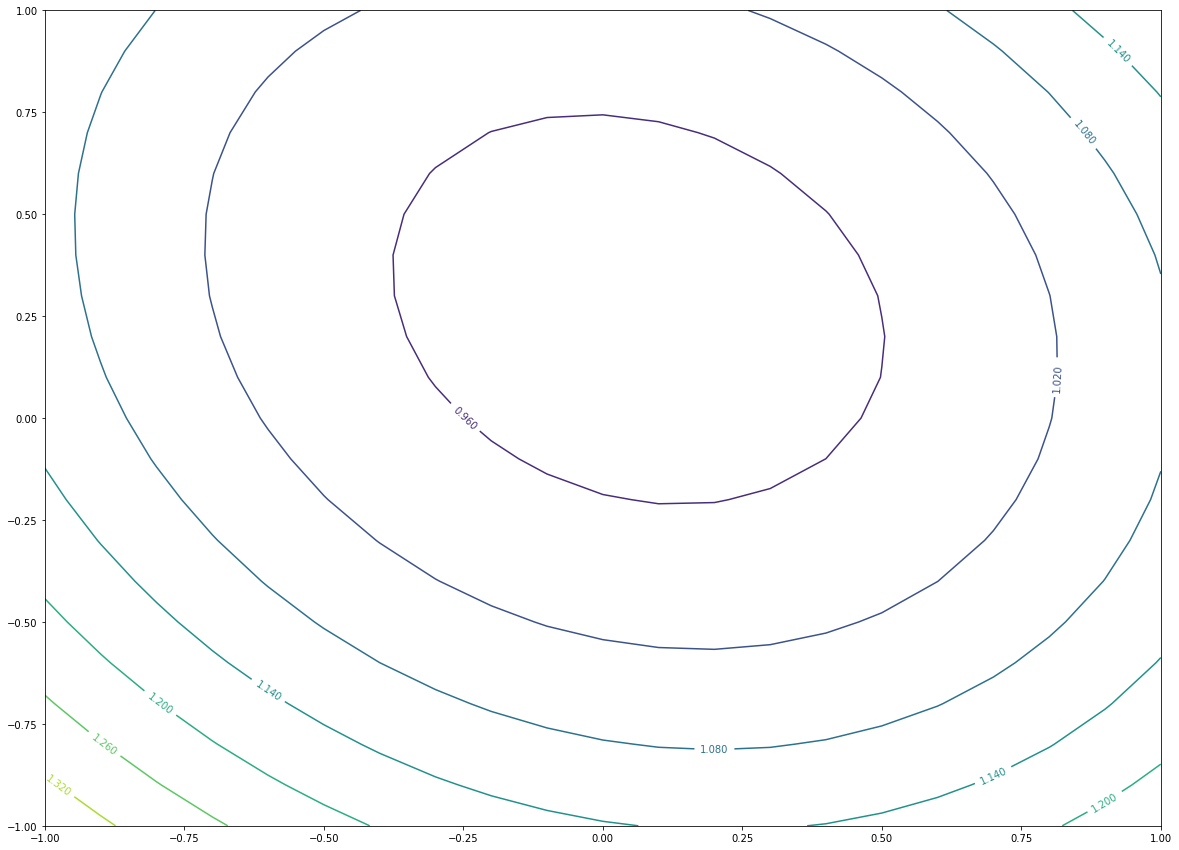
\includegraphics[width=0.49\textwidth]{img/loss_modif_ReNet.png}
	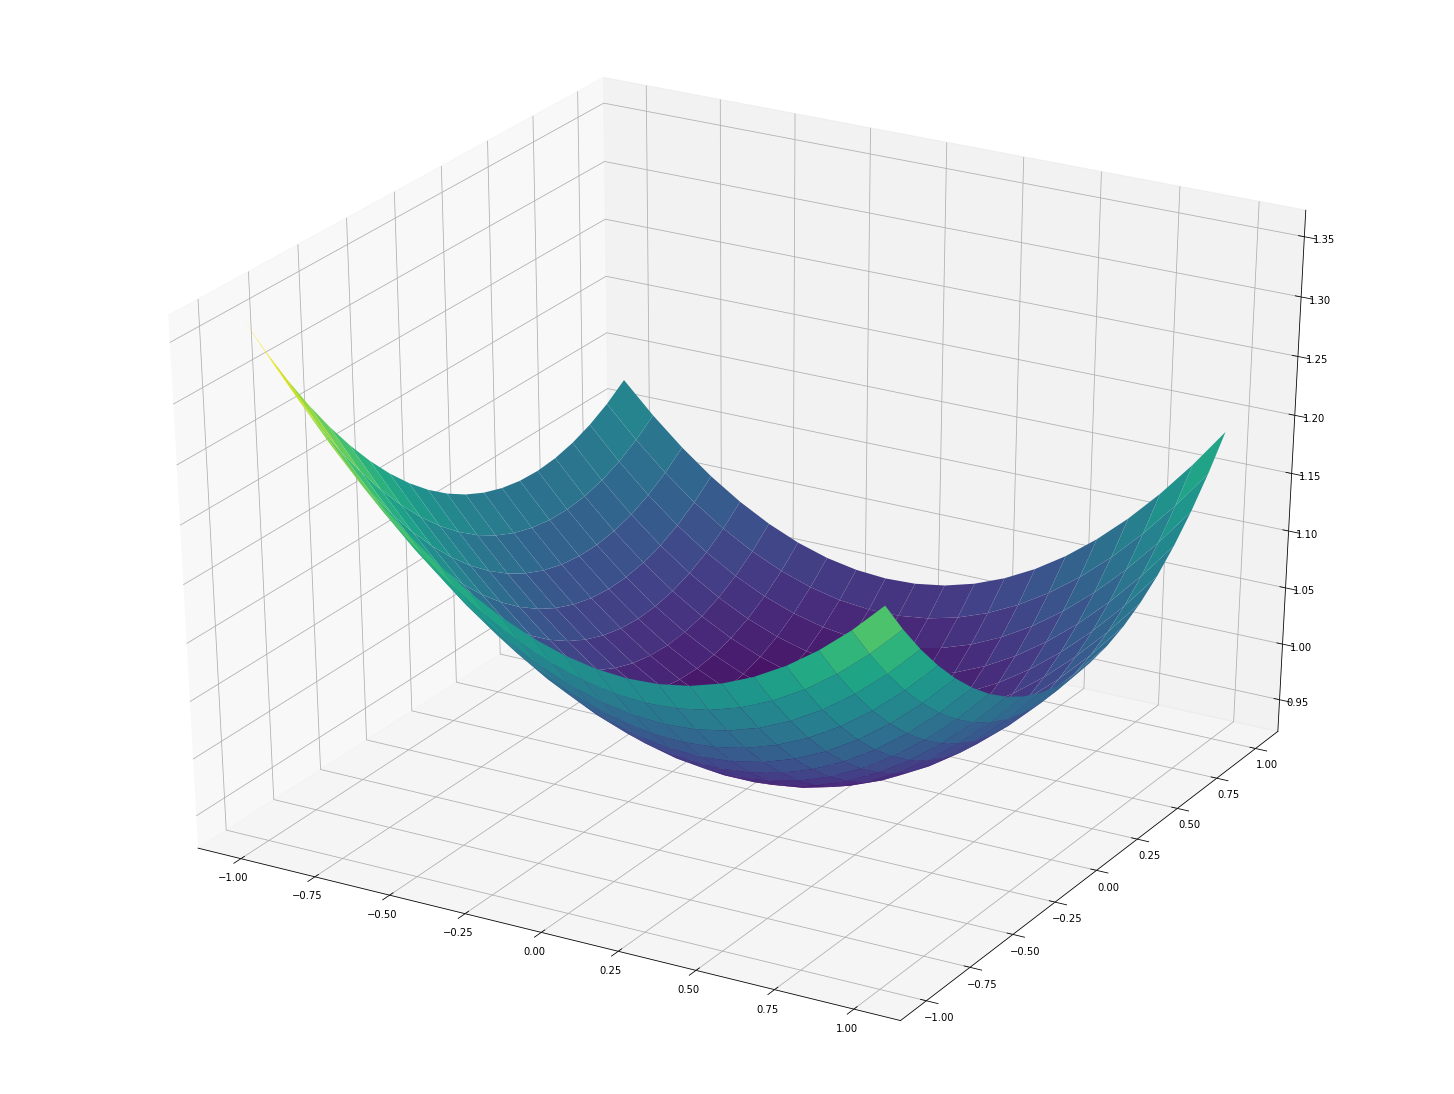
\includegraphics[width=0.49\textwidth]{img/loss_3d_modif_ReNet.png}
	\caption{Visualization of loss landscape of modified ReNet network}
	\label{fig:loss_modif_ReNet}
\end{figure*}

Also based on the loss landscape visualization method introduced in \cite{DBLP:journals/corr/abs-1712-09913} plot of loss value around learned network parameters were prepared. Loss was evaluated based on test set of flowers dataset. Results are shown in figures \ref{fig:loss_ReNet} and \ref{fig:loss_modif_ReNet}.

\section{CONCLUSIONS}

Based on the qualitative results one can say, that convulutional neural networks achieve better accuracy then ReNet and ReNet with modfication. In 3 out of 4 used datasets modified ReNet obtained similar or better results then ReNet. In for Natural Images dataset ReNet outperformes ReNet with modification. For the last dataset some issues were observed and 7 layers of ReNet with modification were need. This shows, that modification introduced in this paper is applicable to all datasets. Introducing modification yielded in substantial speedup for the same datasets, where no performance decrease was noted.

In the tSNE visualization for convolutional network each class forms unified cluster with the exception of few outliers. Based on provided plot one can assume, that each class is easily linearly separable from another. Only mixed classes are 2 and 3. This classes correspond to dog and cat, while other are for example flower, car or airplane. In given situation it is reasonable why cat and dog classes are perceived as similar compared to other classes. The same cannot be found for ReNet networks. Learned representation for both ReNet and ReNet with modification are not linearly separable. There are some Fragments of representation, where one of classes is dominant, but all labels are mixed up. This may be reason why classification task is difficult for ReNet networks.

Assuming that the loss landscape visualization plots are representative one may assume, that ReNet networks have obtained minimum. This minimum can be global or local. If minimum is global, then ReNet networks are not able of achieving minimums with low value that is close to loss obtained by convolutional networks. However results discussed in \cite{Goodfellow-et-al-2016} provide, that deep networks rarely obtain global minimum. Most of the times achived minimum is local, but the value of loss is sufficiently low. One of possibilities is that ReNet networks require some special optimization techniques.

One may ask if speedup obtained is sufficient to provide more practical use for ReNet networks. In case of this studies convolutional networks still obtain better results. Further research in order to improve accuracy and reduce training time of ReNet are required.

Code used for perforing tests is avaliable online in \cite{repo}.


\bibliographystyle{unsrt}
\bibliography{refs}

\end{document}
